% !TeX root = RJwrapper.tex
\title{The R Package \pkg{smicd}: Statistical Methods for Interval-Censored Data}
\author{by Paul Walter}

\maketitle

\abstract{
The package allows the use of two new statistical methods for the analysis of interval-censored data: 1) direct estimation/prediction of statistical indicators and 2) linear (mixed) regression analysis. Direct estimation of statistical indicators, for instance, poverty and inequality indicators, is facilitated by a non parametric kernel density algorithm. The algorithm is able to account for weights in the estimation of statistical indicators. The standard errors of the statistical indicators are estimated with a non parametric bootstrap. Furthermore, the package offers statistical methods for the estimation of linear and linear mixed regression models with an interval-censored dependent variable, particularly random slope and random intercept models. Parameter estimates are obtained through a stochastic expectation-maximization algorithm. Standard errors are estimated using a non parametric bootstrap in the linear regression model and by a parametric bootstrap in the linear mixed  regression model. To handle departures from the model assumptions, fixed (logarithmic) and data-driven (Box-Cox) transformations  are incorporated into the algorithm. 
}

\section{Introduction}

Interval-censored or grouped data occurs when only the lower $A_{k-1}$ and upper  $A_{k}$ interval bounds $(A_{k-1},A_{k})$ of a variable are observed, and its true value remains unknown. Instead of measuring the variable of interest on a continuous scale, for instance, income data,  the scale is divided into $n_{k}$ intervals. The variable $k$ $(1\leq k \leq n_{k})$ indicates in which of the $n_{k}$ intervals an observation falls into. This leads to a loss of information since the shape of the distribution within the intervals remains unknown. In the field of survey statistics, asking for interval-censored data is often done in order to avoid item non-response and thus increase data quality. Item non-response is avoided because interval-censored data offers a higher level of data privacy protection \citep{Hagenaars1988, Moore2000}. Among others, popular surveys and censuses that collect interval-censored data are the German Microcensus \citep{Sta17}, the Colombian census \citep{Dep05}, and the Australian census \citep{Aus11}. While item non-response is reduced or avoided, the statistical analysis of the data requires more elaborate mathematical methods. Even statistical indicators that are easily calculated for metric data, e.g., the mean, cannot be estimated using standard formulas \citep{Fah11}. Also, estimating linear and linear mixed regression models, which are applied in many fields of statistics, requires advanced statistical methods when the dependent variable is interval censored. Therefore, the presented R package implements three major functions: \code{kdeAlgo()} to estimate statistical indicators (e.g., the mean) from interval-censored data, \code{semLm()}, and \code{semLme()} to estimate linear and linear mixed regression models with an interval-censored dependent variable. The package code and the open-source contribution guidelines for the package are available on \href{https://github.com/chiquadrat/smicd}{GitHub}. Potential code contributions, feature requests, and bugs can be reported there by creating issues.

For the estimation of statistical indicators from interval-censored data, different approaches are described in the literature. These approaches can be broadly categorized into four groups: Estimation on the midpoints \citep{Fah11},  linear interpolation of the distribution function, non parametric modeling via splines \citep{Ber16}, and fitting a parametric distribution function to the censored data \citep{Dag77, Mcd84, Ban02}. Some of these methods are implemented in R packages available on the Comprehensive R Archive Network (CRAN). The method of linear interpolation is implemented for the estimation of quantiles in the R package \CRANpkg{actuar} \citep{Dut08a, Dut08b}. The package also enables the estimation of the mean on the interval midpoints. Fitting a parametric distribution to interval-censored data can be done by using the R package \CRANpkg{fitdistrplus} \citep{Del15a, Del15b}. 

In survey statistics, interval-censored data is often collected for income or wealth variables. Thus, the performance of the above-mentioned methods is commonly evaluated by simulation studies that rely on data that follows some kind of income distribution. The German statistical office (DESTATIS) uses the method of linear interpolation for the estimation of statistical indicators from interval-censored income data collected by the German Microcensus. This approach gives the same results as assuming a uniform distribution within the income intervals. Estimation results are reasonably accurate if the estimated indicators do not depend on the whole shape of the distribution, e.g., the median \citep{Len16}. Fitting a parametric distribution to the data enables the estimation of indicators that rely on the whole shape of the distribution. This method works well when the data is censored to only a few equidistant intervals \citep{Len16}. Non parametric modeling via splines shows especially good results for a high number of intervals in ascending order \citep{Len16}.  However, according to \citet{Len16}, all of the above-mentioned methods show large biases and variances when the estimation is based on a small number of intervals. Therefore, a novel kernel density estimation (KDE) algorithm is implemented in the \CRANpkg{smicd} package that overcomes the drawbacks of the previously mentioned methods \citep{Wal19, Wal20}. The algorithm bases the estimation of statistical indicators on pseudo samples that are drawn from a fitted non parametric distribution. The method automatically adapts to the shape of the true unknown distribution and provides reliable estimates for different interval-censoring scenarios. It can be applied via the function \code{kdeAlgo()}.


Similar to the direct estimation of statistical indicators from interval-censored data, there exists a variety of ad-hoc approaches and explicitly formulated mathematical methods for the estimation of linear regression models with an interval-censored dependent variable. The following methods and approaches are used for handling interval-censored dependent variables within linear regression models: Ordinary least squares (OLS) regression on the midpoints \citep{Tho03}, ordered logit- or probit-regression \citep{McC80}, and regression methodology formulated for left-, right-,  and interval-censored data \citep{Tob58, Ros75, Ste83}. All of these methods are implemented in different R packages available on CRAN. OLS regression on the midpoints is applicable by using the \code{lm()} function from the \CRANpkg{stats} package \citep{Cor20}, ordered logit regression is implemented in the \CRANpkg{MASS} package \citep{Rip19, Ven02}, and interval regression is implemented in the \CRANpkg{survival} \citep{Ter20, Ter00} package.



While OLS regression on the midpoints of the intervals is easily applied, it comes with the disadvantage of giving biased estimation results \citep{Cam87}. This approach disregards the uncertainty stemming from the unknown true distribution of the data within the intervals, and therefore, leads to biased parameter estimates. Its performance relies on the number of intervals, and estimation results are only comparable to more advanced methods when the number of intervals is very large \citep{Fry72}. Conceptualizing the model as an ordered logit or probit regression is feasible by treating the dependent variable as an ordered factor variable \citep{McC80}. However, this approach also neglects the unknown distribution of the data within the intervals. Furthermore, the predicted values are not on a continuous scale but are in terms of the probability of belonging to a certain group. To overcome these disadvantages and obtain unbiased estimation results \citet{Ste83} introduces regression methodology for models with an interval-censored dependent variable. \cite{Wal19} further develops his approach and introduces a novel stochastic expectation-maximization (SEM) algorithm for the estimation of linear regression models with an interval-censored dependent variable that is implemented in the \pkg{smicd} package. The model parameters are unbiasedly estimated as long as the model assumptions are fulfilled. The function \code{semLm()} provides the SEM algorithm and enables the use of fixed (logarithmic) and data-driven (Box-Cox) transformations \citep{Box64}. The Box-Cox transformation automatically adapts to the shape of the data and transforms the dependent variable in order to meet the model assumption.

In order to analyze longitudinal or clustered data (e.g., students within schools), linear mixed regression models are applicable. These kinds of models control for the correlated structure of the data by including random effects in addition to the usual fixed effects. In order to deal with an interval-censored dependent variable in linear mixed regression models, there are several approaches described in the literature. Linear mixed regression models, just like linear regression models, can be estimated on the interval midpoints of the censored-dependent variable. Furthermore, conceptualizing the model as an ordered logit or probit regression model is feasible \citep{Agr10}. These approaches inherit the same advantages and disadvantages as previously discussed. Linear mixed regression on the midpoints can be applied by the \CRANpkg{lme4} \citep{Dou20, Dou15} or \CRANpkg{nlme} \citep{Pin20} package and the ordered logit regression is implemented in the \CRANpkg{ordinal} package \citep{Chr15}. To my knowledge, there are no R packages for the estimation of linear mixed regression models with an interval-censored dependent variable. Therefore, the package \pkg{smicd} contains the SEM algorithm proposed by \citet{Wal19} for the estimation of linear mixed regression models with an interval-censored dependent variable. If the model assumptions are fulfilled, the method gives unbiased estimation results. The function \code{semLme()} enables the estimation of the regression parameters, and it also allows for the usage of the logarithmic and Box-Cox transformation in order to fulfill the model assumptions \citep{Gur06}.


The paper is structured into two main sections. Section \ref{Sec:DirectR} deals with the direct estimation of statistical indicators from interval-censored data, whereas Section \ref{Sec:RegressionR} introduces linear and linear mixed regression models with an interval-censored dependent variable. Both sections have been divided into three subsections: first, the statistical methodology is introduced, then the core functions of the \pkg{smicd} package are presented, and finally, illustrative examples with two different data sets are provided. In Section \ref{Sec:DisR}, the main results are summarized, and an outlook is given.


\section{Direct estimation of statistical indicators}\label{Sec:DirectR}

In the following three subsections, the methodology for the direct estimation of statistical indicators from interval-censored data is introduced, the core functionality of the function \code{kdeAlgo()} is presented, and statistical indicators are estimated using the synthetic EU-SILC (European Union Statistics on Income and Living Conditions) data set from Austria.

\subsection{Methodology: Direct estimation of statistical indicators}

In order to estimate statistical indicators from interval-censored data, the proposed algorithm generates metric pseudo samples of an interval-censored variable. These pseudo samples can be used to estimate any statistical indicator. They are drawn from a non parametrically estimated kernel density. Kernel density estimation was first introduced by \citep{Rosenblatt1956} and \citep{Parzen1962}. By  its application, the density \(f(x)\) of a continuous independently and identically distributed random variable is estimated without assuming any distributional shape of the data. The estimator is defined as: 
\begin{equation*}
            \hat{f}_{h}(x) =\frac{1}{nh}\sum_{i=1}^{n}
                           K\left( \dfrac{x-x_i}{h}  \right), \qquad i=1, \ldots, n,
                                        \label{Eq:KerneldefR}
\end{equation*}
where $K\left(\cdot\right)$ is a kernel function, \(h>0\) the bandwidth, and \(x=\{x_{1},x_{2},\ldots,x_{n}\}\) denotes a sample of size \(n\). The performance of the estimator is determined by the optimal choice of \(h\). The selection of an optimal \(h\) is widely discussed in the literature; see \citet{Jon96, Loa99, Zam12}. When working with interval-censored data, a standard KDE cannot be applied since \(x\) is not observed on a continuous scale. Nevertheless, its unobserved true distribution is of continuous form. As an ad hoc solution, the density \(\hat{f}_{h}\left(x\right)\) can be estimated based on the interval midpoints. The resulting density estimate will be spiky unless the bandwidth is sufficiently large. A large bandwidth, however, leads to a loss of information \citep{Wan13}.  Therefore, \citet{Wal19} proposes an iterative KDE algorithm for density estimation from interval-censored data. The approach is based on \citet{Gro17}, who introduce a similar KDE algorithm in a two-dimensional setting with an equidistant interval width. \citet{Wal19} shows that the algorithm can  be adjusted to one-dimensional data with an arbitrary class width. For the estimation of linear and non-linear statistical indicators, the unknown distribution of \(x\) has to be reconstructed by using the observed interval \(k=\{k_{1}, k_{2}, \ldots ,k_{n}\}\) that an observation falls into. From Bayes' theorem \citep{Bay63}, it follows that the conditional distribution of \(\left(x|k\right)\) is:
\begin{equation*}
\pi\left(x|k\right)\propto \pi\left(k|x\right)\pi\left(x\right), 
\end{equation*}
with \(\pi \left(k|x\right)\) is defined by a product of a Dirac distribution \(\pi\left(k|x\right)=\prod_{i=1}^{n}\pi\left(k_{i}|x_{i}\right)\) with
\begin{equation*}
\pi\left(k_{i}|x_{i}\right)=\begin{cases}
  1  & \text{if } A_{k_{i}-1} \leq x_{i} \leq A_{k_{i}}, \\ 
  0 & \text{else, } 
\end{cases}
\end{equation*}
for \(i=1,\ldots,n\). Since \(\pi\left(x\right)\) is unknown, it is replaced by a kernel density estimate \(\hat{f}_{h}\left(x\right)\). 

\subsection{Estimation and computational details}

To fit the model, pseudosamples of \(x_{i}\) are drawn from the conditional distribution
\begin{equation*}
\pi\left(x_{i}|k_{i}\right) \propto \textbf{I}\left(A_{k_{i}-1} \leq x_{i} \leq A_{k_{i}}\right) f\left(x_{i}\right),
\end{equation*}
where \(\textbf{I}\left(\cdot\right)\) denotes the indicator function. The conditional distribution of \(\pi\left(x_{i}|k_{i}\right)\) is given by the product of a uniform distribution and density \(f\left(x_{i}\right)\). As the density is unknown, it is replaced by an estimate \(\hat{f}_{h}\left(x\right)\), which is obtained by the KDE. In particular, \(x_{i}\) is repeatedly drawn from the given interval \(\left(A_{k_{i}-1}, A_{k_{i}}\right)\) by using the current density estimate \(\hat{f}_{h}\left(x\right)\) as a sampling weight. The explicit steps of the iterative algorithm as given in \citet{Wal19} are stated below:
\begin{enumerate}
\item Use the midpoints of the intervals as pseudo \(\tilde{x}_{i}\) for the unknown \(x_{i}\). Estimate a pilot estimate of \(\hat{f}_{h}\left(x\right)\) by applying KDE. Note: Choose a sufficiently large bandwidth \(h\) in order to avoid rounding spikes.
\item Evaluate \(\hat{f}_{h}\left(x\right)\) on an equal-spaced grid \(G=\{g_{1}, \ldots , g_{j}\}\) with  grid points \(g_{1}, \ldots ,g_{j}\). The width of the grid is denoted by \(\delta _{g}\). It is given by
\begin{equation*}
\delta _{g} = \frac{|A_{0}-A_{n_{k}}|}{j-1},
\end{equation*}
and the grid is defined as:
\begin{equation*}
G=\{g_{1}=A_{0}, g_{2}=A_{0}+\delta _{g},g_{3}= A_{0}+2\delta _{g}, \ldots , g_{j-1}=A_{0}+\left(j-2\right)\delta _{g}, g_{j}=A_{n_{k}} \}.
\end{equation*}


\item Sample from \(\pi\left(x|k\right)\) by drawing randomly from \(G_k=\{g_j| g_j\in \left(A_{k-1},A_k\right)\} \) with sampling weights \(\hat{f}_{h}\left(\tilde{x}_{i}\right)\) for \(k=1, \ldots ,n_{k}\). The sample size for each interval is given by the number of observations within each interval. Obtain \(\tilde{x}_{i}\) for \(i=1,\ldots ,n\).
\item Estimate any statistical indicator of interest \(\hat{I}\) using \(\tilde{x}_{i}\).
\item Recompute the density \(\hat{f}_{h}\left(x\right)\) using the pseudo samples \(\tilde{x}_{i}\) obtained in iteration Step 3.
\item Repeat Steps 2-5, with \(B^{(KDE)}\) burn-in and \(M^{(KDE)}\) additional iterations.
\item Discard the \(B^{(KDE)}\) burn-in iterations and estimate the final \(\hat{I}\) by averaging the obtained \(M^{(KDE)}\) estimates.

\end{enumerate}
For open-ended intervals, e.g., \(\left(15000,+\infty\right)\), the upper bound has to be replaced by a finite number. \citet{Wal19} shows through model-based simulations that a value of three times the value of the lower bound \(\left(15000,45000\right)\) gives appropriate estimation results when working with income data.

The variance of the statistical indicators is estimated by bootstrapping. Bootstrap methods were first introduced by \citet{Efr79}. These methods serve as an estimation procedure when the variance cannot be stated as a closed-form solution \citep{Sha95}. While bootstrapping avoids the problem of the non-availability of a closed-form solution, it comes with the disadvantage of long computational times. In the package, a non parametric bootstrap that accounts for the additional uncertainty coming from the interval-censored data is implemented. This non parametric bootstrap is introduced in \citet{Wal19}. 


\subsection{Core functionality: Direct estimation of statistical indicators}\label{Sec:DirectCoreR}

The presented KDE algorithm is implemented in the function \code{kdeAlgo()} (see Table \ref{Tab:CoreDirectR}). The arguments and default settings of  \code{kdeAlgo()}  are briefly summarized in Table \ref{Tab:ArgkdeAlgoR}. The function gives back an S3 object of class \code{"kdeAlgo"}. A detailed explanation of all components of a \code{"kdeAlgo"} object can be found in the package documentation. The generic functions \code{plot()} and \code{print()} can be applied  to \code{"kdeAlgo"} objects to output the main estimation results (see Table \ref{Tab:CoreDirectR}). In the next section, the function \code{kdeAlgo()} is used to estimate a variety of statistical indicators from interval-censored EU-SILC data, and its arguments are explained in more detail.


\begin{table}[ht]
\caption{Implemented functions for the direct estimation of statistical indicators.}
\label{Tab:CoreDirectR}
\centering
\begin{tabular}{ ll }
\toprule
Function Name & Description \\
\midrule
\code{kdeAlgo()} & Estimates the statistical indicators and its standard errors from \\
&interval-censored data\\
\code{plot()} & Plots convergence of the estimated statistical indicators and   \\
& estimated density of the pseudo $\tilde{x}_{i}$\\ 
\code{print()} & Prints the estimated statistical indicators and its standard errors\\
\bottomrule
\end{tabular}
\end{table}



\begin{table}[ht]
\caption{Arguments of function \code{kdeAlgo()}.}
\label{Tab:ArgkdeAlgoR}
\centering
\begin{tabular}{ lll }
\toprule
Argument & Description & Default \\
\midrule
\code{xclass}	& Interval-censored variable & \\
\code{classes}	& Numeric vector of interval bounds & \\
\code{threshold} &	Threshold used for poverty indicators & \\
&  (\% of the median of the target variable)  &  \code{0.6} \\
\code{burnin}	& Number of burn-in iterations \(B^{(KDE)}\) & \code{80}\\
\code{samples}	& Number of additional iterations \(M^{(KDE)}\) & \code{400}\\
\code{bootstrap.se} & If TRUE, standard errors of the statistical \\
&indicators are estimated & \code{FALSE}\\
\code{b} & Number of bootstraps for the estimation of \\
& the standard errors & \code{100} \\
\code{bw}	&  Smoothing bandwidth used & \code{"nrd0"}\\
\code{evalpoints} &	Number of evaluation grid points & \code{4000} \\
\code{adjust} & Bandwidth multiplier \(bw=adjust*bw\) & \code{1} \\
\code{custom\_indicator} & A list of user-defined statistical indicators &  \code{NULL}  \\
\code{upper} & If upper bound of the upper interval is \(+\infty\), e.g.,  & \\
& \((15000,+\infty)\), then \(+\infty\) is replaced by  &  \\
& \(15000*upper\) & \code{3} \\
\code{weights} & Survey weights & \code{NULL} \\
\code{oecd} & Household weights of equivalence scale & \code{NULL} \\
\bottomrule
\end{tabular}
\end{table}


\subsection{Example: Direct estimation of statistical indicators}\label{Sec:DirectExampleR}

To demonstrate the function \code{kdeAlgo()}, the  equivalized household income and the corresponding household sample weight from the Austrian synthetic EU-SILC survey data set are used. The data set is included in the \CRANpkg{laeken} package \citep{Tem20, Tem13}. Its synthetic nature makes it unusable for inferential statistics. However, the data set has the advantage over the scientific use file by being freely available which enables the easy reproducibility of the presented example. Since the total disposable household income is measured on a continuous scale, it is censored to 22 intervals for demonstration purposes. For a realistic censoring scheme, the interval bounds are chosen such that they closely follow the interval bounds used in the German Microcensus from 2013 \citep{Sta14}. The German Microcensus is a representative household survey that covers 830,000 persons in 370,000 households (1\% of the German population) in which income is only collected as an interval-censored variable \citep{Sta16}. 
 
In a first step, the variable total disposable household income called \code{hhincome\_net} is interval-censored according to 22 intervals using the function \code{cut()}. The vector of interval bounds is called \code{intervals}, and  the newly obtained interval-censored income variable is called \code{c.hhincome}. 

\begin{example}
R> intervals <- c(
+    0, 150, 300, 500, 700, 900, 1100, 1300, 1500, 1700, 2000, 2300, 2600, 2900, 
+    3200, 3600, 4000, 4500, 5000, 5500, 6000, 7500, Inf
+  )
R> c.hhincome <- cut(hhincome_net, breaks = intervals)
\end{example}

In order to get a descriptive overview of the distribution of the censored income data, the function \code{table()}  is applied.


\begin{example}
R> table(c.hhincome)
c.hhincome
          (0,150]         (150,300]         (300,500] 
               66               113               280 
        (500,700]         (700,900]     (900,1.1e+03] 
              462              1137              1433 
(1.1e+03,1.3e+03] (1.3e+03,1.5e+03] (1.5e+03,1.7e+03] 
             2040              1811              1671 
  (1.7e+03,2e+03]   (2e+03,2.3e+03] (2.3e+03,2.6e+03] 
             2006              1383               849 
(2.6e+03,2.9e+03] (2.9e+03,3.2e+03] (3.2e+03,3.6e+03] 
              508               389               242 
  (3.6e+03,4e+03]   (4e+03,4.5e+03]   (4.5e+03,5e+03] 
              158               107                61 
  (5e+03,5.5e+03]   (5.5e+03,6e+03]   (6e+03,7.5e+03] 
               21                18                52 
    (7.5e+03,Inf]
               17
\end{example}

Most incomes are in interval $(1100,1300]$, and only 17 incomes are in the upper interval. For the estimation of the statistical indicators, the function \code{kdeAlgo()} of the \pkg{smicd} package is called with the following arguments. 

\begin{example}
R> Indicators <- kdeAlgo(
+    xclass = c.hhincome, classes = intervals, 
+    bootstrap.se = TRUE, custom_indicator = 
+     list(
+      quant05 = function(y, threshold, weights) {
+       wtd.quantile(y, probs = 0.05, weights)
+      }, 
+      quant95 = function(y, threshold, weights) {
+       wtd.quantile(y, probs = 0.95, weights)
+      }
+     ), 
+    weights = hhweight
+  )
\end{example}

The variable \code{c.hhincome} is assigned to the argument \code{xclass}, and the vector of interval bounds \code{intervals} is assigned to the argument \code{classes}. The default settings of the arguments \code{burnin}, \code{samples}, \code{bw}, \code{evalpoints}, \code{adjust}, and \code{upper} are retained. Simulation results from \citet{Wal19} and \citet{Gro17} show that these settings give good results when working with income data. Changing these arguments has an impact on the performance of the KDE algorithm. As default, the statistical indicators: mean, Gini coefficient, headcount ratio (HCR),  the quantiles (10\%, 25\%, 50\%, 75\%, 90\%), the poverty gap (PGAP), and the quintile share ratio (QSR) are estimated \citep{Gin12, Fos84}. The HCR and PGAP rely on a poverty threshold. The default choice of the \code{threshold} argument is 60\% of the median of the target variable, as suggested by \citet{Eur14}. Besides the mentioned indicators, any other statistical indicator can be estimated via the argument \code{custom\_indicator}. In the example, the argument is assigned a list that holds functions to estimate the 5\% and 95\% quantile. The custom indicators must depend on the target variable, the threshold (even if it is not needed for the specified indicator), and optionally on the weights argument if the estimation of a weighted indicator is required. To estimate the standard errors of all indicators, \code{bootstrap.se = TRUE}, and the number of bootstrap samples is 100 (the default value as suggested in \citet{Wal19}).  Lastly, the household weight (\code{hhweight}) is assigned to the argument \code{weights} in order to estimate weighted statistical indicators. It can also be controlled for households of different sizes by assigning \code{oecd} a variable with household equivalence weights. By applying the \code{print()} function to the \code{"kdeAlgo"} object, the estimated statistical indicators (default and custom indicators) as well as their standard errors are printed. For instance, in this example, the estimated mean is about 1,658 Euro and its standard error is 8.486.

\begin{example}
R> print(Indicators)
Value:
    mean   gini    hcr  quant10   quant25   quant50  
1658.329  0.265  0.145  802.227  1117.714  1507.947 
 quant75   quant90   pgap     qsr  quant05   quant95 
 2020.063 2654.707  0.040   3.920  630.326  3142.296  

Standard error:
   mean   gini    hcr quant10 quant25 quant50 
  8.486  0.002  0.002   5.839   5.977   6.605  
quant75 quant90   pgap    qsr quant05 quant95 
 10.548  21.622  0.001  0.044  10.327  24.401 
\end{example}

For demonstration purposes, the statistical indicators are also estimated using the continuous household income variable from the synthetic EU-SILC data set (Table \ref{Tab:directEst}). The estimation results of the KDE algorithm using the interval-censored data are very close to those based on the continuous data. Slightly larger deviations are observable for the more extreme quantiles. This is due to the fact that these quantile estimates fall into intervals with a lower number of observations (compared to the other quantile estimates). Estimation results for these quantiles could potentially be further improved by increasing the number of \code{evalpoints} of the \code{kdeAlgo()}.

\begin{table}[ht]
\caption{Estimated weighted statistical indicators using the continuous household income variable from the synthetic EU-SILC data set.}
\label{Tab:directEst}
\centering
\begin{tabular}{ rrrrrrr }
\toprule
\code{mean} & \code{gini} & \code{hcr} & \code{quant10} & \code{quant25} & \code{quant50}\\
1657.910 & 0.265 & 0.144 & 805.468 & 1114.028 & 1508.657\\
\midrule
\code{quant75} & \code{quant90} & \code{pgap} & \code{qsr} & \code{quant05} & \code{quant95}\\
2017.585 & 2653.617 & 0.040 & 3.960 & 619.666 & 3153.425 \\
\bottomrule
\end{tabular}
\end{table}

In \citet{Wal19}, the performance of the KDE algorithm is evaluated via detailed simulation studies. By applying the function \code{plot()},  \code{"kdeAlgo"} objects can be plotted. Thereby, convergence plots for all estimated statistical indicators and a plot of the estimated final density are obtained. 

\begin{example}
R> plot(Indicators)
\end{example}


Figure \ref{Fig:kdeAlgoConv} shows convergence plots for two of the estimated indicators. Additionally, a plot of the estimated final density with a histogram of the observed data in the background is given in Figure \ref{Fig:kdeAlgoDens}. In Figure \ref{Fig:kdeAlgoConv}, the estimated statistical indicator (Gini, 10\% quantile)  for each iteration step of the KDE algorithm and the average over the estimates up to iteration step M (excluding the burn-in iterations) are plotted. A vertical line marks the end of the burn-in period. The horizontal line gives the value of the final estimate (average over the M iterations). All convergence plots indicate that the number of iterations is chosen sufficiently large for the estimates to converge. 

If convergence were not achieved, the arguments \code{burnin} and \code{samples} should be increased. It is notable that the estimated 10\% quantile has the same value for almost all iterations steps. This is the case because the quantile, as any other statistical indicator, is estimated using the pseudo samples that are drawn on 4,000 grid points $G$. Estimating a quantile on only 4,000 unique outcomes (pseudo values) leads to equal quantile estimates for numerous iteration steps of the KDE algorithm.


\begin{figure}[ht]
  \centering
    \includegraphics[width=0.9\textwidth]{Gini.pdf}
     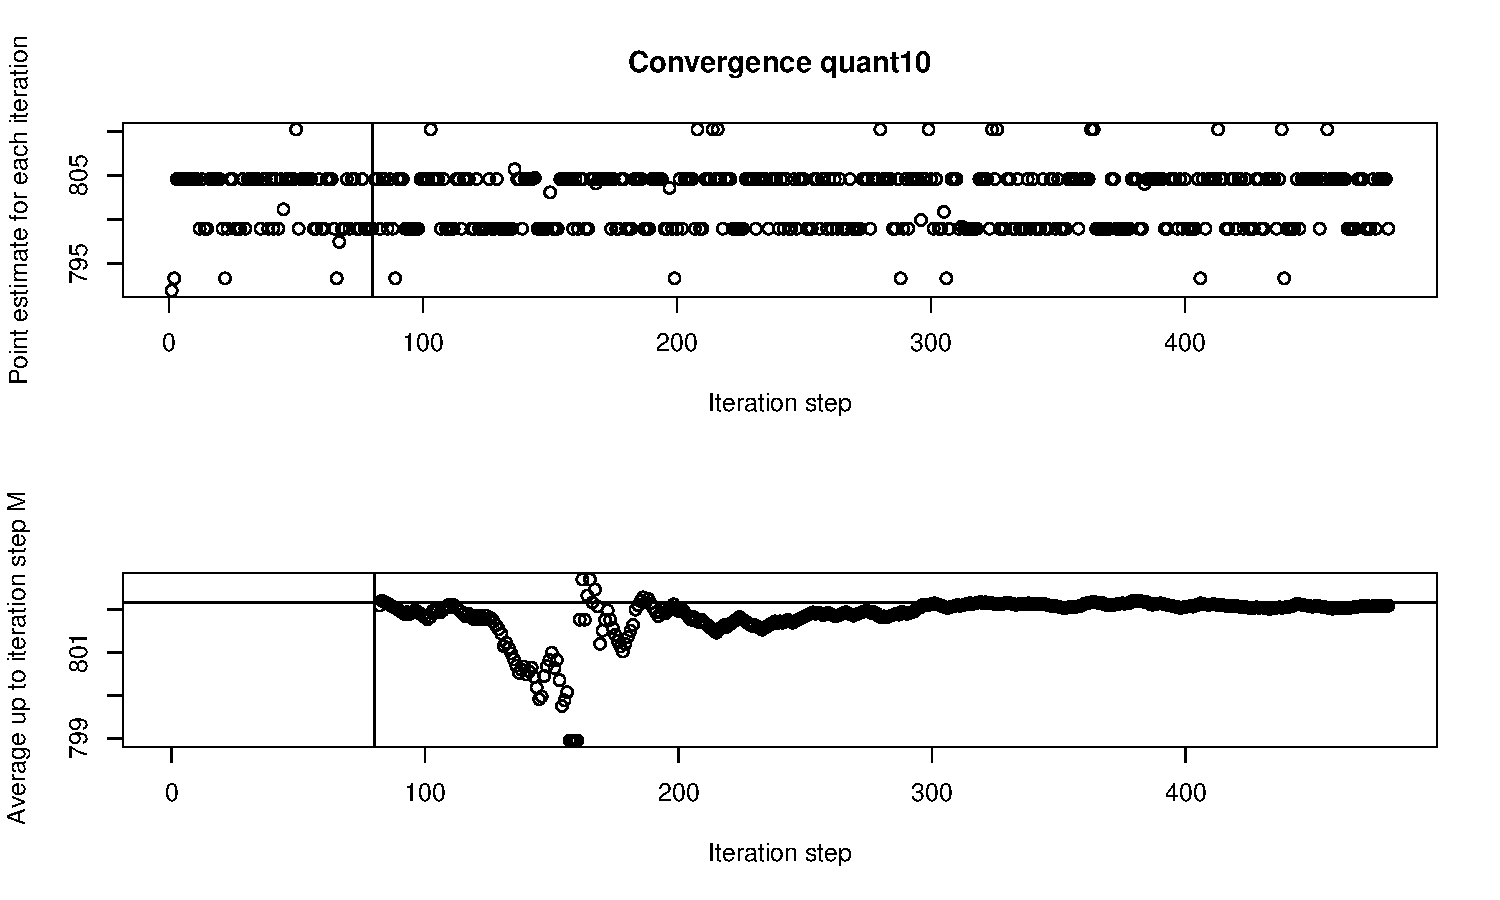
\includegraphics[width=0.9\textwidth]{quant10.pdf}
     \caption{Convergence plots of the estimated indicators (Gini and 10\% quantile).}
     \label{Fig:kdeAlgoConv}
\end{figure}

\begin{figure}[ht]
  \centering
     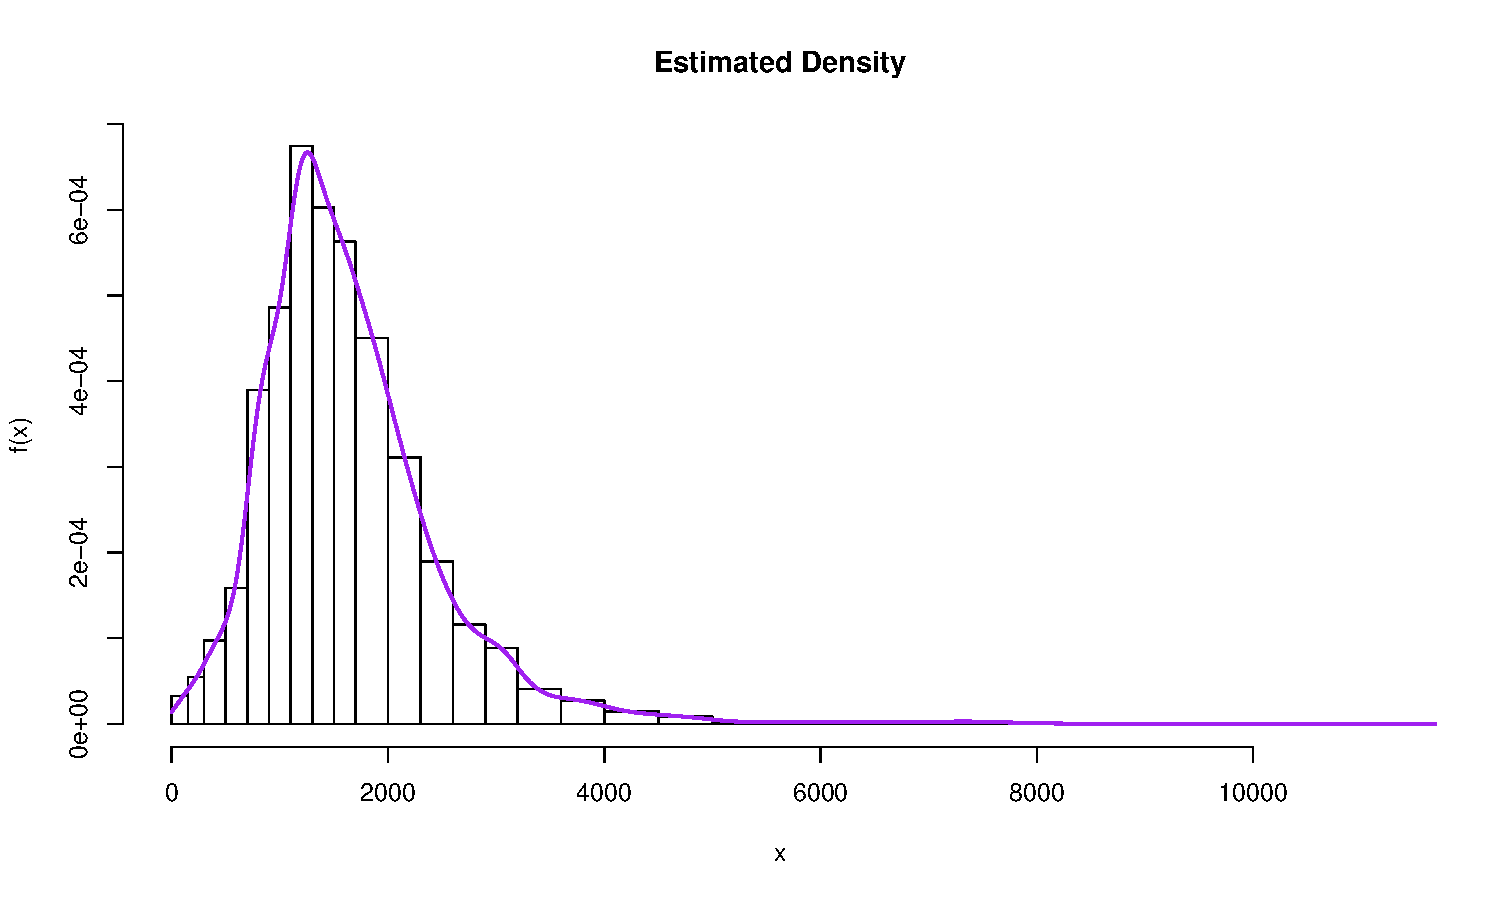
\includegraphics[width=0.9\textwidth]{densKDE.pdf}
     \caption{Estimated final density with a histogram of the observed distribution of the data in the background.}
     \label{Fig:kdeAlgoDens}
\end{figure}

Lastly, it should be mentioned that the computation time can be very long if the estimation of the standard errors is enabled. Hence, if the estimation of the standard errors is not required, the argument \code{bootstrap.se} should be set to \code{FALSE}. Furthermore, it should always be checked how many iterations are needed for the desired statistical indicator to converge. Reducing the number of required iterations (arguments \code{burnin} and \code{samples}) lowers the computation time significantly (with and without standard errors).

\section{Regression analysis}\label{Sec:RegressionR}

In the following three subsections, the statistical methodology for linear and linear mixed regression models with an interval-censored dependent variable is introduced, the core functionality of the functions \code{semLM()} and \code{semLME()} is presented, and  examination scores of students from schools in London are exemplary modeled.

\subsection{Methodology: Regression analysis}

The theoretical introduction of the new regression method, proposed by \citet{Wal19}, is presented for linear mixed  regression models. The theory for linear regression models can be obtained by simplifying the introduced method. In its standard form, the linear mixed regression model serves to analyze the linear relationship between a continuous dependent variable and some independent variables \citep{Gol03}. Random parameters (random slopes and random intercepts) are included in the model to account for correlated data, e.g., students within schools.  The model in matrix notation \citep{Lai83} is given by
\begin{equation}
\label{Eq:NestedErrorModelR}
\mathbf{y}=\mathbf{X}\boldsymbol{\beta}+\mathbf{Z}\mathbf{v}+\mathbf{e},
\end{equation}
where \(\mathbf{y}\) is an \(n \times 1\) column vector of the dependent variable, \(n\) is the sample size, \(\mathbf{X}\) is a \(n \times p\) matrix where \(p\) is equal to the number of predictors, \(\boldsymbol{\beta}\) is a column vector of the fixed effects regression parameters of size \(p \times 1\), \(\mathbf{Z}\) is the \(n\times q\) design matrix with \(q\) random effects, \(\mathbf{v}\) is a \(q \times 1\) vector of random effects, and \(\mathbf{e}\) is the residual vector of size \(n\times 1\). The distribution of the random effects is given by
\begin{equation*}
\mathbf{v}\sim N\left(\mathbf{0}, \mathbf{G}\right), \qquad \text{ where } \mathbf{G}=\begin{bmatrix}
\sigma_{0}^{2}	& \sigma_{01}	& \dots	 & \sigma_{0q}      \\
\sigma_{10}	& \sigma_{1}^{2} 	& \dots  & \sigma_{1q} 	  \\
\vdots	& \vdots 	& \ddots & \vdots \\
\sigma_{q0} 	& \sigma_{q1} & \dots	 & \sigma_{q}^{2}
\end{bmatrix},
\end{equation*}
and the distribution of the residuals is given by \(\mathbf{e}\sim N\left(\mathbf{0},\mathbf{R}\right)\) with \(\mathbf{R}=\mathbf{I}_{n}\sigma_{e}^{2}\), where \(\mathbf{I}_{n}\) is the identity matrix, and \(\sigma^{2}_{e}\) is the residual variance. The random effects \(\mathbf{v}\) and the residuals \(\mathbf{e}\) are assumed to be independent. For a more detailed introduction of mixed models, see \citet{Sea92, McC08, Sni11}. In the case of an interval-censored dependent variable, the parameters of Model (\ref{Eq:NestedErrorModelR}) have to be estimated without observing \(\mathbf{y}\) on a continuous scale. Instead, only the interval identifier \(\mathbf{k}\), now defined as \(n\times 1\) column vector, is observed. Open-ended interval bounds \(A_{0}=-\infty \)  and \(A_{n_{k}}=+\infty\) and unequal interval widths are allowed. Since the true distribution of \(\mathbf{y}\) is unknown, the aim is to reconstruct the distribution of \(\mathbf{y}\)  using the known intervals  \(\mathbf{k}\) and the linear relationship stated in Model (\ref{Eq:NestedErrorModelR}). As presented in \citet{Wal19}, in order to reconstruct the unknown distribution of \(f\left(\mathbf{y}|\mathbf{X}, \mathbf{Z}, \mathbf{v}, \mathbf{k}, \boldsymbol{\theta}\right)\), where \(\boldsymbol{\theta} = \left(\boldsymbol{\beta},\mathbf{R}, \mathbf{G}\right)\), the Bayes theorem \citep{Bay63} is applied. Hence,
\begin{equation*}
f\left(\mathbf{y}|\mathbf{X}, \mathbf{Z}, \mathbf{v}, \mathbf{k}, \boldsymbol{\theta}\right) \propto f\left(\mathbf{k}|\mathbf{y}, \mathbf{X}, \mathbf{Z}, \mathbf{v}, \boldsymbol{\theta}\right)f\left(\mathbf{y}|\mathbf{X}, \mathbf{Z}, \mathbf{v}, \boldsymbol{\theta}\right),
\end{equation*}
with \(f\left(\mathbf{k}|\mathbf{y}, \mathbf{X}, \mathbf{Z}, \mathbf{v}, \boldsymbol{\theta}\right)=f\left(\mathbf{k}|\mathbf{y}\right)\) because the conditional distribution of the interval identifier \(\mathbf{k}\) only depends on \(\mathbf{y}\). It is given by \(f\left(\mathbf{k}|\mathbf{y}\right)=\mathbf{r}\), with \(\mathbf{r}\) being an \(n \times 1\) column vector \(\mathbf{r}=\left(r_{1},r_{2}, \ldots , r_{n} \right)^{T} \), with 
\begin{equation*}
r_{i}=\begin{cases}
  1  & \text{if } A_{k_{i}-1} \leq y_{i} \leq A_{k_{i}}, \\ 
  0 & \text{else, }
\end{cases}
\end{equation*}
for \(i=1, \ldots, n\) and 
\begin{equation}
\label{Eq:distR}
f\left(\mathbf{y}|\mathbf{X}, \mathbf{Z}, \mathbf{v}, \boldsymbol{\theta}\right)  \sim \enspace N\left(\mathbf{X}\boldsymbol{\beta}+\mathbf{Z}\mathbf{v}, \mathbf{R}\right). 
\end{equation}
The relationship in Equation (\ref{Eq:distR}) follows from the linear mixed model assumptions (Model (\ref{Eq:NestedErrorModelR})). The unknown parameters  \(\boldsymbol{\theta}=\left(\boldsymbol{\beta},\mathbf{R},\mathbf{G}\right)\) are estimated based on pseudo samples \(\mathbf{\tilde{y}}\) (since \(\mathbf{y}\) is unknown) that are iteratively drawn from  \(f\left(\mathbf{y}|\mathbf{X}, \mathbf{Z}, \mathbf{v}, \mathbf{k}, \boldsymbol{\theta}\right)\). The next subsection states the computational details of the SEM algorithm.

\subsection{Estimation and computational details}

To fit  Model (\ref{Eq:NestedErrorModelR}), the parameter vector \(\boldsymbol{\hat{\theta}}=\left(\boldsymbol{\widehat{\beta}},\mathbf{\widehat{R}},\mathbf{\widehat{G}}\right)\) is estimated, and pseudo samples of the unknown \(\mathbf{y}\) are iteratively generated by the following SEM algorithm. The pseudo samples \(\mathbf{\tilde{y}}\) are drawn from the conditional distribution 
\begin{equation*}
f\left(\mathbf{y}|\mathbf{X}, \mathbf{Z}, \mathbf{v},\mathbf{k} ,\boldsymbol{\theta}\right) \propto \textbf{I}\left(A_{\mathbf{k}-1} \leq \mathbf{y} \leq A_{\mathbf{k}}\right) \times N\left(\mathbf{X}\boldsymbol{\beta}+\mathbf{Z}\mathbf{v}, \mathbf{R}\right),
\end{equation*}
where \(\textbf{I}\left(\cdot\right)\) denotes the indicator function. Hence, for \(\mathbf{y}\) with explanatory variables \(\mathbf{X}\), the corresponding \(\mathbf{\tilde{y}}\) is drawn from \(N\left(\mathbf{X}\boldsymbol{\beta}+\mathbf{Z}\mathbf{v}, \mathbf{R}\right)\) conditional on the given interval \(\left(A_{\mathbf{k}-1} \leq \mathbf{y} \leq A_{\mathbf{k}}\right)\). If \(\boldsymbol{\hat{\theta}}\) is estimated, the conditional distribution \(f\left(\mathbf{y}|\mathbf{X}, \mathbf{Z}, \mathbf{v},\mathbf{k} ,\boldsymbol{\theta}\right)\) follows a two-sided truncated normal distribution. Its probability density function equals
\begin{equation}
\label{Eq:TwoTruncR}
\hat{f}\left(\mathbf{y}|\mathbf{X}, \mathbf{Z}, \mathbf{\hat{v}}, \mathbf{k}, \boldsymbol{\hat{\theta}}\right)=\frac{\phi\Big(\frac{\mathbf{y}-\boldsymbol{\hat{\mu}}}{\hat{\sigma}_{e}}\Big)}{\hat{\sigma}_{e}\bigg(\Phi \Big(\frac{A_{\mathbf{k}}-\boldsymbol{\hat{\mu}}}{\hat{\sigma}_{e}}\Big)-\Phi \Big(\frac{A_{\mathbf{k}-1}-\boldsymbol{\hat{\mu}}}{\hat{\sigma}_{e}}\Big)\bigg)},
\end{equation}
with \(\boldsymbol{\hat{\mu}} = \mathbf{X}\widehat{\boldsymbol{\beta}}+\mathbf{Z}\mathbf{\hat{v}}\).  \(\phi\left(\cdot\right)\) denotes the probability density function of the standard normal distribution, and \(\Phi(\cdot)\) denotes its cumulative distribution function. From its definition, it follows that \(\Phi \Big(\frac{A_{\mathbf{k}}-\boldsymbol{\hat{\mu}}}{\hat{\sigma}_{e}}\Big) = 1\) if \(A_{\mathbf{k}}=+\infty \), and \(\Phi \Big(\frac{A_{\mathbf{k}-1}-\boldsymbol{\hat{\mu}}}{\hat{\sigma}_{e}}\Big)=0\) if \(A_{\mathbf{k}-1}=-\infty\). The steps of the SEM algorithm as described in \citet{Wal19} are:
\begin{enumerate}
\item Estimate \(\boldsymbol{\hat{\theta}}=\left(\boldsymbol{\widehat{\beta}},\mathbf{\widehat{R}},\mathbf{\widehat{G}}\right)\)  from Model (\ref{Eq:NestedErrorModelR}) using the midpoints of the intervals as substitutes for the unknown \(\mathbf{y}\). The parameters are estimated by restricted maximum likelihood theory (REML) \citep{Tho62}.

\item \textbf{Stochastic step:} For  \(i=1,\ldots , n\), draw randomly from \(N\left(\mathbf{X}\boldsymbol{\widehat{\beta}}+\mathbf{Z}\mathbf{\hat{v}}, \mathbf{\widehat{R}}\right)\) within the given interval \(\left(A_{\mathbf{k}-1} \leq \mathbf{y} \leq A_{\mathbf{k}}\right)\) (the two-sided truncated normal distribution given in Equation (\ref{Eq:TwoTruncR})) obtaining \(\left(\mathbf{\tilde{y}},\mathbf{X},\mathbf{Z}\right)\). The drawn pseudo \(\mathbf{\tilde{y}}\) are used as replacements for the unobserved \(\mathbf{y}\).

\item \textbf{Maximization step:} Re-estimate the parameter vector \(\boldsymbol{\hat{\theta}}\) from Model (\ref{Eq:NestedErrorModelR}) by using the pseudo samples \(\left(\mathbf{\tilde{y}},\mathbf{X},\mathbf{Z}\right)\) from Step 2. Again, parameter estimation is carried out by REML.

\item Iterate Steps 2-3 \(B^{(SEM)}+M^{(SEM)}\) times, with \(B^{(SEM)}\) burn-in iterations and \(M^{(SEM)}\)  additional iterations. 

\item Discard the burn-in iterations \(B^{(SEM)}\) and estimate \(\boldsymbol{\hat{\theta}}\) by averaging the obtained \(M^{(SEM)}\) estimates.

\end{enumerate} 
If open-ended intervals \(A_{0}=-\infty \) and \(A_{n_{k}}=+\infty \) are present, the midpoints \(M_{1}\) and \(M_{n_{k}}\) of these intervals in iteration Step 1 are computed as follows:
\begin{equation*}
\begin{split}
M_{1}&=\left(A_{1}-\overline{D}\right)/2, \\
M_{n_{k}}&=\left(A_{n_{k}-1}+\overline{D}\right)/2,
\end{split}
\end{equation*}
where
\begin{equation*}
\overline{D}=\frac{1}{\left(n_{k}-2\right)}\sum_{k=2}^{n_{k}-1}|A_{k-1}-A_{k}|.
\end{equation*}
These midpoints serve as proxies for the unknown interval midpoints in Step 1 of the algorithm.  The SEM algorithm for the linear regression model is obtained by simplifying the conditional distribution \(f\left(\mathbf{y}|\mathbf{X}, \mathbf{Z}, \mathbf{v}, \boldsymbol{\theta}\right)  \sim \enspace N\left(\mathbf{X}\boldsymbol{\beta}+\mathbf{Z}\mathbf{v}, \mathbf{R}\right)\) to \(f\left(\mathbf{y}|\mathbf{X},\boldsymbol{\beta}, \sigma_{e}^{2}\right) \sim N\left(\mathbf{X}\boldsymbol{\beta}, \sigma_{e}^{2}\right)\) according to the model assumptions of a linear regression model. In the  SEM algorithm for linear models, it is then drawn from \(N\left(\mathbf{X}\boldsymbol{\beta}, \sigma_{e}^{2}\right)\) within the given interval. 

The standard errors of the regression parameters are estimated using bootstrap methods. For the linear regression model, a non parametric bootstrap \citep{Efr81, Efr82, Efr86, Efr93} and for the linear mixed regression model, a parametric bootstrap \citep{Wan06, Tha13} is used to estimate the standard errors. The non parametric, as well as the parametric bootstrap, are further developed to account for the additional uncertainty that is due to the interval-censored dependent variable.  Both newly proposed bootstraps are available in the \pkg{smicd} package, and the theory is explained in \citep{Wal19}.

To assure that the model assumptions are fulfilled, the logarithmic and the Box-Cox transformations are incorporated into the function \code{semLm()} and \code{semLme()}. 



\subsection{Core functionality: Regression analysis}\label{Sec:RegressionCoreR}

The introduced SEM algorithm is implemented in the functions described in Table \ref{Tab:CoreSEMR}. The arguments and default settings of the estimation functions \code{semLm()} and \code{semLme()} are summarized in Table \ref{Tab:semR}. Both functions return an S3 object of class \code{"sem"}, \code{"lm"} or \code{"sem"}, \code{"lme"}. A detailed explanation of all the components of these objects can be found in the \pkg{smicd} package documentation. The generic functions \code{plot()}, \code{print()}, and \code{summary()} can be applied  to objects of class \code{"sem", "lm"} and \code{"sem", "lme"} in order to summarize the main estimation results. In the next section, the functionality of \code{semLm()} and \code{semLme()} is demonstrated based on an illustrative example.

\begin{table}[ht]
\caption{Implemented functions for the estimation of linear and linear mixed regression models.}
\label{Tab:CoreSEMR}
\centering
\begin{tabular}{ ll }
\toprule
Function Name & Description \\
\midrule
\code{semLm()} & Estimates linear regression models with an interval-censored  \\
&    dependent variable\\
\code{semLme()} & Estimates linear mixed regression models with an  \\
&interval-censored dependent variable\\
\code{plot()} & Plots convergence of the estimated parameters and estimated   \\
& density of the pseudo $\mathbf{\tilde{y}}$ from the last iteration step\\ 
\code{print()} & Prints basic information of the estimated linear and linear mixed  \\
& regression models\\
\code{summary()} & Summary of the estimated linear and linear mixed regression models\\ 
\bottomrule
\end{tabular}
\end{table}



\begin{table}[ht]
\caption{Arguments of functions \code{semLm()} and \code{semLme()}.}
\label{Tab:semR}
\centering
\begin{tabular}{ lll }
\toprule
Argument & Description & Default \\
\midrule
\code{formula}	& A two-sided linear formula object & \\
\code{data}	& A data frame containing the variables of the model & \\
\code{classes} & Numeric vector of interval bounds & \\
\code{burnin} &	Burn-in iterations &  \code{40}  \\
\code{samples}	& Additional iterations & \code{200}\\
\code{trafo} & Transformation of the dependent variable: None, & \code{"None"}\\
& logarithmic, or Box-Cox transformation & \\
\code{adjust} & Extends the number of iterations for the estimation  & \code{2}  \\
&  of the Box-Cox transformation parameter:  &  \\
&\((burnin+samples)*adjust\)& \\
\code{bootstrap.se} & If TRUE, standard errors and confidence intervals of & \code{FALSE}\\
&the regression parameters are estimated &  \\
\code{b}	&  Number of bootstraps for the estimation of \\
& the standard errors & \code{100}\\
\bottomrule
\end{tabular}
\end{table}

\subsection{Example: Regression analysis}\label{Sec:RegressionExampleR}

To demonstrate the functions \code{semLm()} and \code{semLme()}, the famous London school data set that is analyzed in \citet{Gol93} is used. The data set contains the examination results of 4,059 students from 65 schools in six Inner London Education Authorities. The data set is available in the R package \CRANpkg{mlmRev} \citep{Bat14} and also included in the package \pkg{smicd}. The variables used in the following example are: general certificate of secondary examination scores (\code{examsc}), the standardized London reading test scores at the age of 11 years (\code{standLRT}), the sex of the student (\code{sex}), and the school identifier (\code{school}). In the original data set, the variable \code{examsc} is measured on a continuous scale. In order to demonstrate the functionality of the functions \code{semLm()} and \code{semLme()}, the variable is arbitrarily censored to nine intervals. As before, the censoring is carried out by the function \code{cut()}, and the vector of interval bounds is called \code{intervals}.

\begin{example}
R> intervals <- c(1, 1.5, 2.5, 3.5, 4.5, 5.5, 6.5, 7.7, 8.5, Inf)
R> Exam$examsc.class <- cut(Exam$examsc, intervals)
\end{example}

The newly created interval-censored variable is called \code{examsc.class}. The distribution is visualized by applying the function \code{table()}.


\begin{example}
R> table(Exam$examsc.class)
  (1,1.5] (1.5,2.5] (2.5,3.5] (3.5,4.5] (4.5,5.5] (5.5,6.5] 
        1        32       249       937      1606       951 
(6.5,7.7] (7.7,8.5] (8.5,Inf] 
      267        15         1
\end{example}
%$

It can be seen that most examination scores are concentrated in the center intervals. To fit the linear regression model, the function \code{semLM()} is called. 

\begin{example}
R> LM <- semLm(
+    formula = examsc.class ~ standLRT + sex, data = Exam, 
+    classes = intervals,  bootstrap.se = TRUE
+  )
\end{example}


The formula argument is assigned the model equation, where \code{examsc.class} is regressed on \code{standLRT} and \code{sex}. The argument \code{data} is assigned the name of the data set \code{Exam}, and the vector of interval bounds \code{intervals} is assigned to the \code{classes} argument. The arguments \code{burnin} and \code{samples} are left as defaults. The specified number of default iterations is sufficiently large for most regression models. However the convergence of the parameters has to be checked by plotting the estimation results with the function \code{plot()} after the estimation. No transformation is specified  for the interval-censored dependent variable and therefore, \code{trafo} is assigned its default value. The argument \code{adjust} is only relevant if the Box-Cox transformation \code{trafo="bc"} is chosen. In this case, the number of iterations for the estimation of the Box-Cox transformation parameter \(\lambda\) can be specified by this argument. The convergence of the transformation parameter \(\lambda \) has to be checked using the function \code{plot()}. More information on the Box-Cox transformation and on the estimation of the transformation parameter is given in \citet{Wal19}. For the estimation of the standard errors of the regression parameters, the argument \code{bootstrap.se} is set to \code{TRUE}. The number of bootstrap samples \code{b} is 100, its default value, which again is reasonable for most settings. A summary of the estimation results is obtained by the application of the function \code{summary()}.

\begin{example}
R> summary(LM)
Call:
semLm(formula = examsc.class ~ standLRT + sex, data = Exam,
     classes = intervals, bootstrap.se = TRUE)

Fixed effects:
             Estimate  Std.Error Lower 95%-level Upper 95%-level
(Intercept) 5.0702791 0.01816102       5.0326739       5.1033905
standLRT    0.5908015 0.01349275       0.5614197       0.6163845
sexM       -0.1715966 0.03093346      -0.2308930      -0.1010877

Multiple R-squared: 0.3501  Adjusted R-squared: 0.3498
Variable examsc.class is divided into 9 intervals.
\end{example}

The output shows the function call, the estimated regression coefficients, the bootstrapped standard errors, and the confidence intervals, as well as the R-squared and the adjusted R-squared. Furthermore, the output reminds the user that the dependent variable is censored to nine intervals. All estimates are interpreted as in a linear regression model with a continuous dependent variable. Hence, if \code{standLRT} increases by one unit and all other parameters are kept constant, \code{examsc.class} increases by 0.59 on average. The bootstrapped confidence intervals indicate that all regressors have a significant effect on the dependent variable.



By using the generic function \code{plot()} on an object of class \code{"sem"} and \code{"lm"}, convergence plots of each estimated regression parameter and of the estimated residual variance are obtained. Furthermore, the density of the generated pseudo \(\mathbf{\tilde{y}}\) variable from the last iteration step is plotted with a histogram of the observed distribution of the interval-censored variable \code{examsc.class} in the background.

\begin{example}
R> plot(LM)
\end{example}

\begin{figure}[ht]
  \centering
    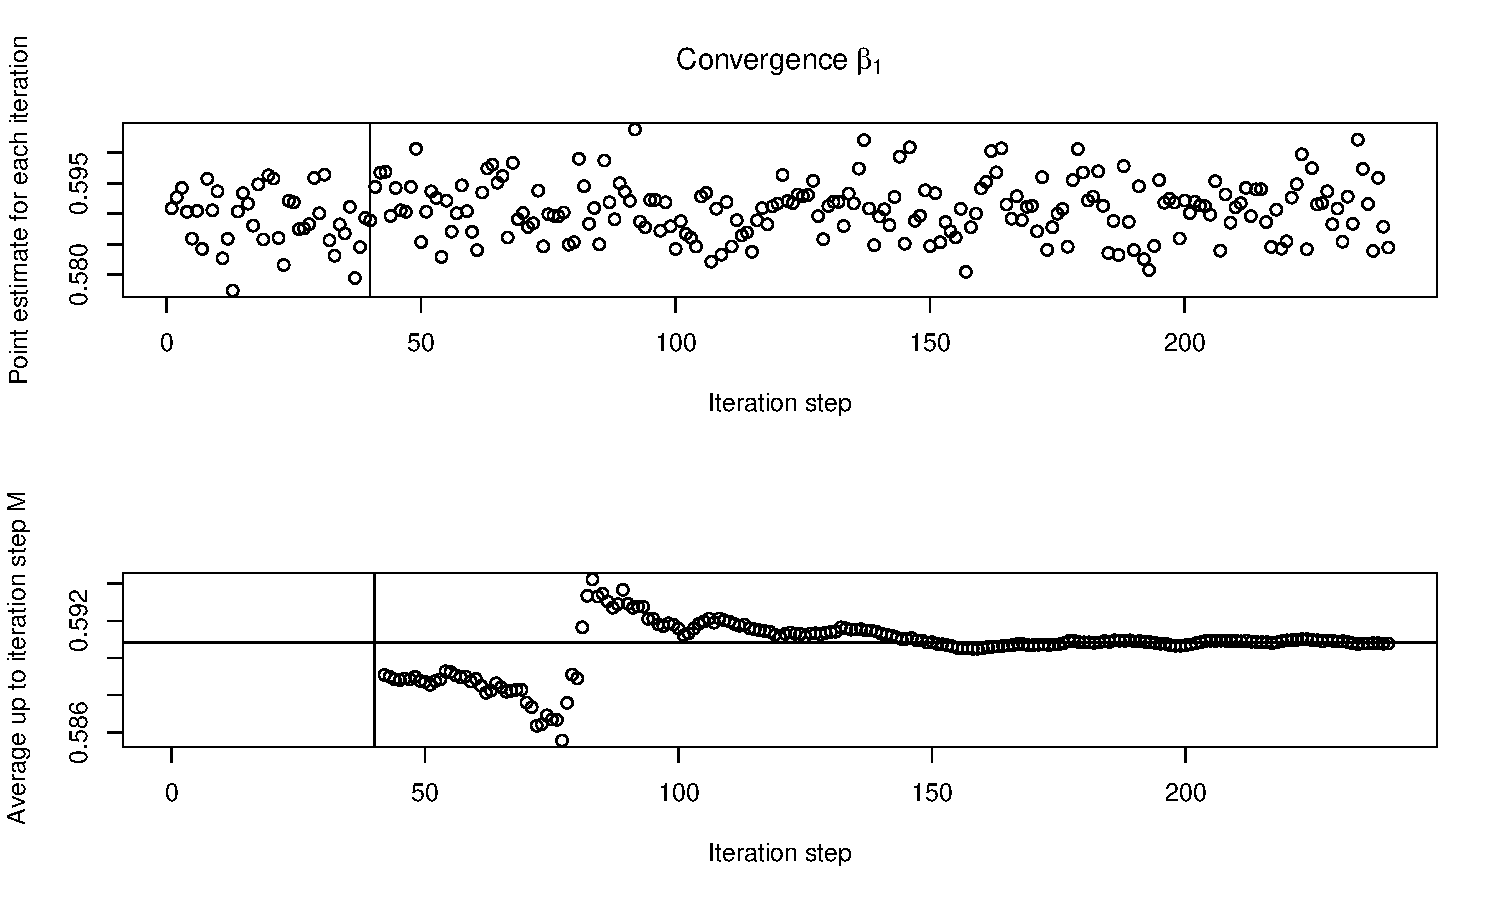
\includegraphics[width=0.9\textwidth]{beta1.pdf}
    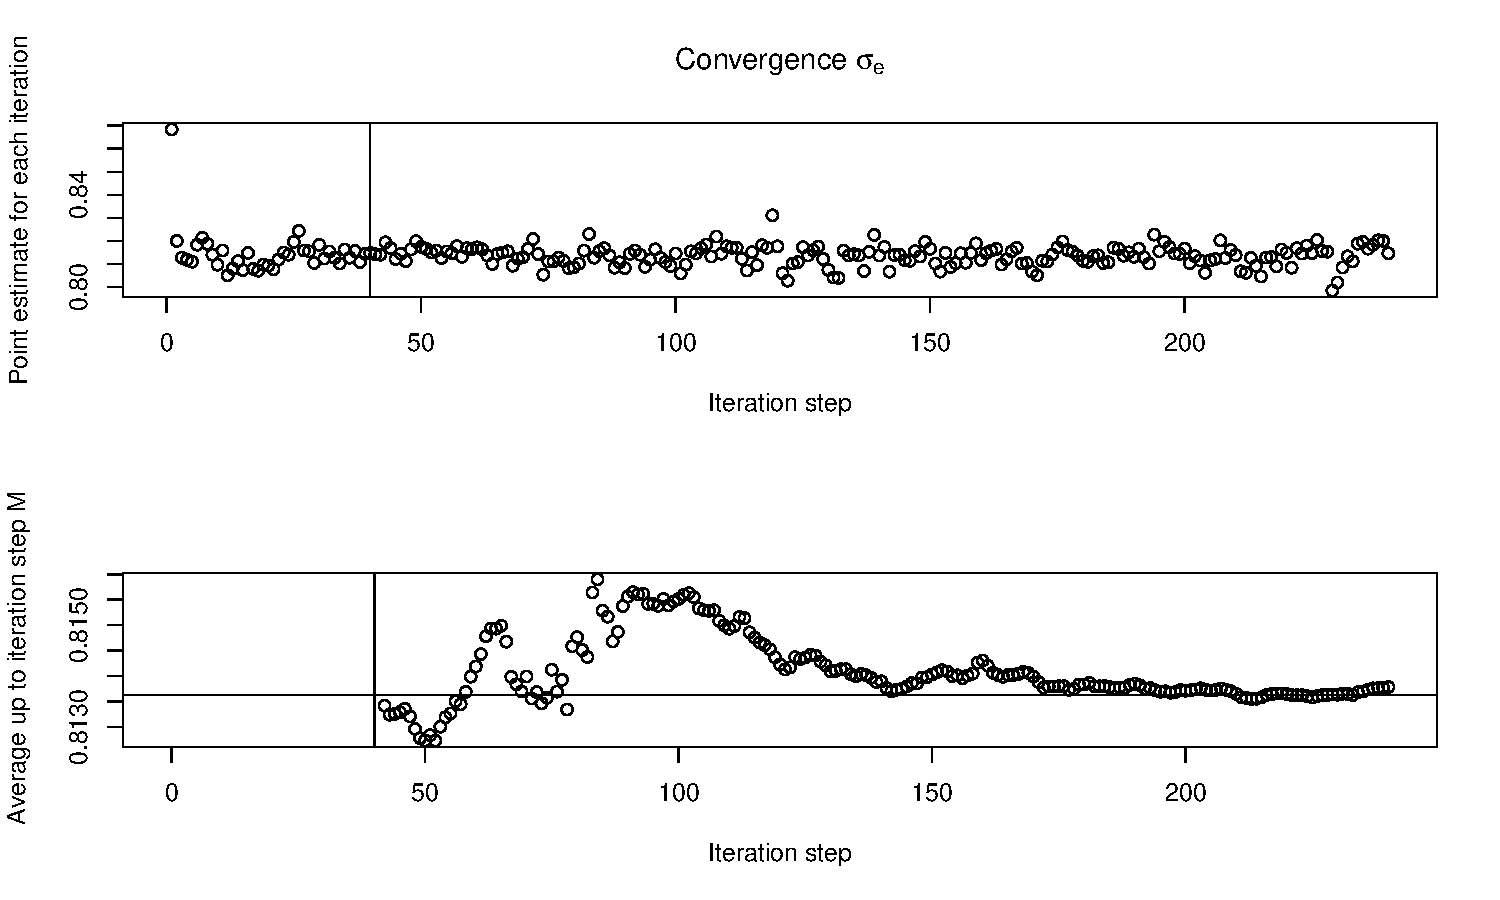
\includegraphics[width=0.9\textwidth]{sigmae.pdf}
     \caption{Convergence plots of estimated model parameters ($\beta_{1}$ and $\sigma_{e}$).}
     \label{Fig:semCon}
\end{figure}

\begin{figure}[ht]
  \centering
    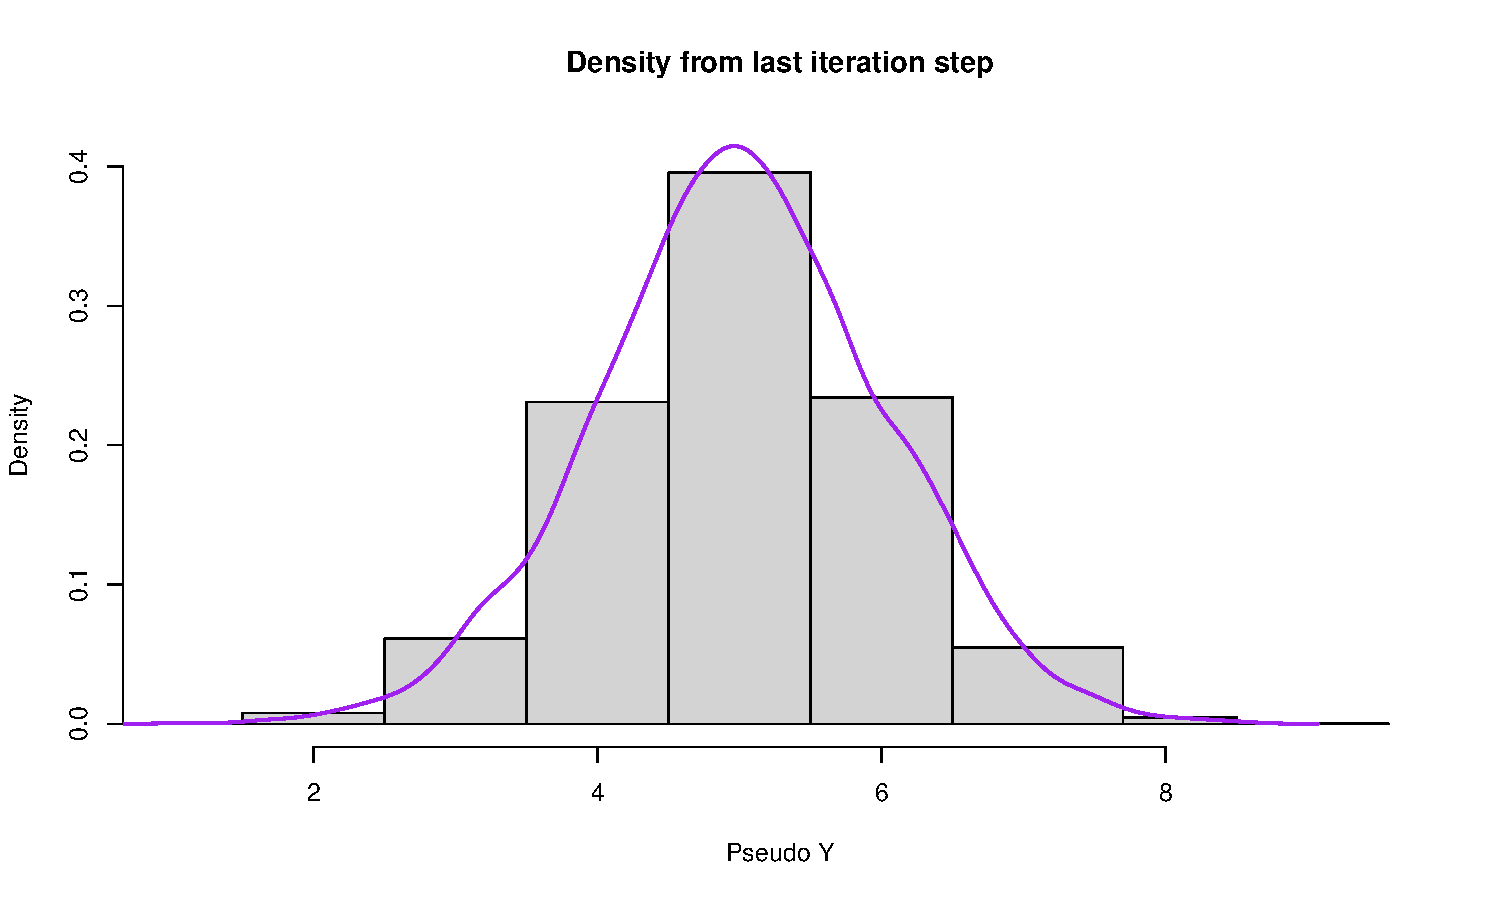
\includegraphics[width=0.9\textwidth]{densReg.pdf}
     \caption{Estimated final density with a histogram of the observed distribution of the data in the background.}
     \label{Fig:semDen}
\end{figure}

In Figure \ref{Fig:semCon}, a selection of convergence plots is given, and in Figure \ref{Fig:semDen}, the density of the pseudo  \(\mathbf{\tilde{y}}\) from the last iteration step of the SEM algorithm is plotted. In the convergence plots, the estimated parameter and the average up to iteration step \(M\) (excluding \(B\)) are plotted for each iteration step of the SEM algorithm. A vertical line indicates the end of the burn-in period (40 iterations). The final parameter estimate marked by the horizontal line is obtained by averaging the \(M^{(SEM)}\) additional iterations (200). The selected 240 iterations are enough to obtain reliable estimates in this example because the estimates have converged.

As already mentioned, the \pkg{smicd} package also enables the estimation of linear mixed regression models by the function \code{semLme()}. In the London school data set, students are nested within schools, and therefore, it is necessary to control for the correlation within-schools. In order to do that, the variable \code{school} is specified as a random intercept. If necessary, a random slope parameter could also be included in the model. Again, the variable \code{sex} is included as an additional regressor. Hence, the \code{formula} argument is assigned the following model equation \code{examsc.class} \(\sim\) \code{standLRT + sex + (1|school)}. So far, the function \code{semLme()} enables the estimation of linear mixed models with a maximum of one random slope and one random intercept parameter. Regarding all other arguments, the same specifications as before are made.

\begin{example}
R> LME <- semLme(
+    formula = examsc.class ~ standLRT + sex + (1|school), 
+    data = Exam, classes = intervals, bootstrap.se = TRUE
+  )
\end{example}

By using the generic function \code{summary()}, the estimation results are printed. In addition to the fixed effects, the estimated random effects are obtained as in the \pkg{lme4} and \pkg{nlme} packages. Since the R-squared and the adjusted R-squared are not defined for mixed models, the \code{summary()} function prints the marginal R-squared and conditional R-squared \citep{Nak13, Joh14}. 

\begin{example}
> summary(LME)
Call:
semLme(formula = examsc.class ~ standLRT + sex + (1 | school), 
    data = Exam, classes = intervals, bootstrap.se = TRUE)
    
Random effects:
    Groups        Name   Variance  Std.Dev.
    school (Intercept) 0.08755431 0.2958958
  Residual             0.58417586 0.7643140

Fixed effects:
             Estimate    Std.Error Lower 95%-level Upper 95%-level
(Intercept) 5.0777581 0.0005188930       5.0769749       5.0791095
standLRT    0.5605049 0.0003665976       0.5599456       0.5613711
sexM       -0.1711065 0.0008159909      -0.1724193      -0.1692369

Marginal R-squared: 0.324 Conditional R-squared: 0.4121
Variable examsc.class is divided into 9 intervals.
\end{example}

Again, interpretation is the same as in linear mixed models with a continuous dependent variable. By applying the generic function \code{plot()} to a \code{"sem" "lme"} object, the same  plots as for the linear regression model are plotted.

\section{Discussion and outlook}\label{Sec:DisR}
Asking for interval-censored data can lead to lower item non-response rates and increased data quality. While item non-response is potentially avoided, applying traditional statistical methods becomes infeasible because the true distribution of the data within each interval is unknown. The  functions of the \pkg{smicd} package enable researchers to easily analyze this kind of data. The paper briefly introduces the new statistical methodology and presents, in detail, the core functions of the package: 
\begin{itemize}
\item \code{kdeAlgo()} for the direct estimation of any statistical indicator,
\item \code{semLm()} to estimate linear models with an interval-censored dependent variable,
\item \code{semLme()} to estimate linear mixed models with an interval-censored dependent variable.
\end{itemize}
The functions are applied in order to estimate statistical indicators from interval-censored synthetic EU-SILC income data and to analyze interval-censored examination scores of students from London with linear and linear mixed regression models.


Further developments of the \pkg{smicd} package will include the possibility to estimate the bootstrapped standard errors in parallel computing environments. Additionally, it is planned to allow for the use of survey weights in the linear (mixed) regression models.



\bibliography{WalterReferences}

\address{Paul Walter\\
  Freie Universität Berlin\\
  Garystraße 21, 14195 Berlin\\
  Germany\\
  \email{paul.walter@fu-berlin.de}}

